\chapter{Proposed Navigation Filter Architecture}
Scalar tracking loops discussed in Chapter~3 are critically important to receivers as they adapt the replica signal to match the receiver signal data for proper decoding. However, these scalar loop filters assume a static noise bandwidth, regardless of receiver or satellite dynamics. If either platforms have unmodeled dynamics unknown before processing, these bandwidths can permit too much noise into the navigation processing solution or, do not allow enough of the signal to be processed, neglecting these dynamics. One solution to this problem is implementing an adaptive Kalman filter to optimally select bandwidths~\cite{}. In this case, the Kalman filter estimates the proper bandwidth based on discriminator residuals, but is agnostic to the dynamics of the receiver or the satellite dynamics. The addition of an adaptive Kalman filter is in an improvement, but leaves a lot to be desired as each channel is still be tracked individually, resulting in low-powered channels having a high likelihood of being lost.

Another, more optimal, solution is to estimate the receiver and satellite dynamics at every integration period. This requires an updated estimate of the navigation solution to be updated at every integration period, which is suitable as long as four satellites are transmitting to the receiver. This approach combines the adaptive bandwidth from~\cite{} along with knowledge of the receiver and satellite dynamics stemming from the navigation solution. This closed-loop approach is known as \textit{vector tracking} and will be discussed in greater detail later on in this chapter. Specifically, the Vector Delay and Frequency Lock Loop (VFDLL) is the vector tracking implementation used in this thesis.

To build on the attractive approach that vector tracking brings to processing received signal data, the novelty of this work proposes an addendum to the existing navigation filter architecture by adding a Flight Vehicle Dynamic Model (FVDM) to predict the trajectory of flight vehicle in time to better assist with the processing of the signal. Along wth the discussion of vector tracking, this chapter will describe the process model in the Extended Kalman Filter (EKF), and the measurement update that provides corrections to estimated state of the receiver in time.
\section{Vector Delay and Frequency Lock Loop}
Vector tracking first utilized a Vector Delay Lock Loop (VDLL) and was proposed by~\cite{}. In a VDLL, the EKF provides continuous estimates of the code frequency, updating the DLL, improving overall tracking performance. Later on,~\cite{}, explores tracking both code frequency and carrier frequency in an EKF, coined the VDFLL. This method showed great improvements over scalar tracking algorithms and moderate improvements over the VDLL. The VFDLL proves best when tracking weaker GNSS signals under high dynamic stress~\cite{}. Furthermore, recent analyses from~\cite{} prove the VFDLL has improved resilance to multipath delay as well. A block diagram of the VFDLL is shown in Figure~\ref{fig:VFDLL}.

\begin{figure}[!ht]
    \centering
    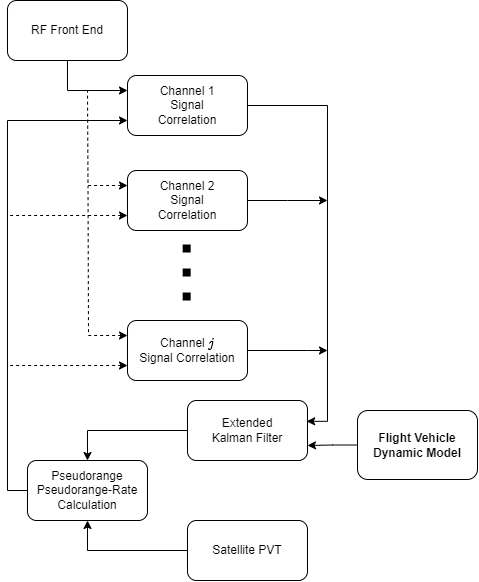
\includegraphics[width=0.45\linewidth]{Figures/VectorTracking.drawio.png}
    \caption{Block diagram of the VFDLL used in this work}\label{fig:VFDLL}
\end{figure}

From Figure~\ref{fig:VFDLL}, the \textit{RF Front End} block refers to the discussion in Section~3.1. The signal correlation block represent Equation~\ref{eq:correlators} and also the the FLL and DLL discriminators specified in Equations~\ref{eq:FLLdisc} and~\ref{eq:DLLdisc}, respectively. The basic flow of the VFDLL requires the receiver to know its position and the positions of the satellites \textit{a priori}. Preferably, initial positions and satellite positions that fed into the VFDLL are from processing the received signal for a length of time required to decode the navigation message using scalar tracking discussed in Chapter 3. The requirements of the EKF in Figure~\ref{fig:VFDLL} are residual pseudorange and pseudorange-rates in the form of outputs from the discriminators. The EKF uses the measurements from the current signal correlations to improve the position estimate of the receiver. Using the ephemeris of the satellites and the corrected position estimates, new code phase and carrier frequency estimates are generated for the next integration period. To improve the estimated position from the EKF, the FVDM is used as the process model to propagate the non-linear motion of the aircraft in time. The next section covers the time update and measurement update within the EKF.
\clearpage
\section{Deeply Coupled GPS and FVDM Navigation Filter}



\begin{equation}\label{eq:eulerIntegration}
    \mathbf{X}_{k} = \dot{\mathbf{X}}\Delta t + \mathbf{X}_{k-1}
\end{equation}

\begin{equation}\label{eq:acc}
    \begin{bmatrix}
        \dot{V_N} \\
        \dot{V_E} \\
        \dot{V_D} \\
    \end{bmatrix} =
    \mathbf{C}_{b}^{n}\frac{\mathbf{f}_{ib}^b}{m} - \left(2\mathbf{\Omega}_{ie}^n - \mathbf{\Omega}_{en}^n\right)
    \begin{bmatrix}
        V_N \\
        V_E \\
        V_D \\
    \end{bmatrix}
\end{equation}

\begin{equation}\label{eq:angacc}
    \begin{bmatrix}
        \dot{p}_{ib}^b \\
        \dot{q}_{ib}^b \\
        \dot{r}_{ib}^b \\
    \end{bmatrix} =
    {\mathbf{I}_{cg}^b}^{-1}\left[\mathbf{M}_{ib}^b -
        \begin{bmatrix}
            p \\
            q \\
            r \\
        \end{bmatrix} \times
        \left(\mathbf{I}_{cg}^b
        \begin{bmatrix}
            p \\
            q \\
            r \\
        \end{bmatrix}
        \right)
        \right]
\end{equation}

\begin{equation}\label{eq:posrate}
    \begin{bmatrix}
        \dot{\lambda}_{eb}^n \\
        \dot{L}_{eb}^n       \\
        \dot{h}_{eb}^n       \\
    \end{bmatrix} =
    \begin{bmatrix}
        \frac{V_N}{R_N + h_{eb}^n}                                       \\
        \frac{V_E}{\left(R_E + h_{eb}^n\right)\cos\left(L_{eb}^n\right)} \\
        -V_D                                                             \\
    \end{bmatrix}\\
\end{equation}

\begin{equation}\label{eq:eulerRates}
    \begin{bmatrix}
        \dot{\phi}_{bn}   \\
        \dot{\theta}_{bn} \\
        \dot{\psi}_{bn}   \\
    \end{bmatrix} =
    \mathbf{C}_{\omega}
    \left(
    \begin{bmatrix}
            p \\
            q \\
            r \\
        \end{bmatrix} -
    \mathbf{C_n^b}\left(\omega_{ie}^n + \omega_{en}^n\right)
    \right)
\end{equation}

\begin{equation}\label{eq:clkRates}
    \begin{bmatrix}
        c\delta \dot{t} \\
        c\delta\ddot{t} \\
    \end{bmatrix} =
    \begin{bmatrix}
        0 & 1 \\
        0 & 0 \\
    \end{bmatrix}
    \begin{bmatrix}
        c\delta {t}    \\
        c\delta\dot{t} \\
    \end{bmatrix}
\end{equation}

\begin{equation}\label{eq:velVector}
    \mathbf{X}_V =
    \begin{bmatrix}
        V_N & V_E & V_D \\
    \end{bmatrix}
\end{equation}

\begin{equation}\label{eq:omegaVector}
    \mathbf{X}_{\omega} =
    \begin{bmatrix}
        p_{ib}^b & q_{ib}^b & r_{ib}^b \\
    \end{bmatrix}
\end{equation}

\begin{equation}\label{eq:posVector}
    \mathbf{X}_P =
    \begin{bmatrix}
        \lambda_{eb}^n & L{eb}^n & h{eb}^n \\
    \end{bmatrix}
\end{equation}

\begin{equation}\label{eq:eulVector}
    \mathbf{X}_{\psi} =
    \begin{bmatrix}
        \phi_{bn} & \theta_{bn} & \psi_{bn} \\
    \end{bmatrix}
\end{equation}

\begin{equation}\label{eq:clkVector}
    \mathbf{X}_t = \begin{bmatrix}
        c\delta t & c\delta\dot{t} \\
    \end{bmatrix}
\end{equation}

\begin{equation}\label{eq:pminus}
    \mathbf{P}^-_{k} = \mathbf{\Phi}\mathbf{P}^-_{k-1} \mathbf{\Phi}^T + \mathbf{Q_d}
\end{equation}

\begin{equation}\label{eq:Qd}
    \mathbf{Q_d} = \mathbf{\Phi}\mathbf{B}_w \left(ww^T\right) \mathbf{B}_w^T \mathbf{\Phi}^T \Delta t
\end{equation}

\begin{equation}\label{eq:w}
    w = \begin{bmatrix}
        w_{dyn} & w_{clk}
    \end{bmatrix}
\end{equation}

\begin{equation}\label{eq:wDyn}
    w_{dyn} = \begin{bmatrix}
        \sigma^2_{V_N} & \sigma^2_{V_E} & \sigma^2_{V_E} & \sigma^2_{p} & \sigma^2_{q} & \sigma^2_{r}
    \end{bmatrix}
\end{equation}

\begin{equation}\label{eq:wClk}
    w_{clk} = \begin{bmatrix}
        \sigma^2_b & \sigma^2_d \\
    \end{bmatrix}
\end{equation}

\begin{equation}\label{eq:Phi}
    \mathbf{\Phi} = \textrm{expm}(\mathbf{F}\Delta t)
\end{equation}

\begin{equation}\label{eq:stateVector}
    \mathbf{X} =
    \begin{bmatrix}
        \mathbf{X}_V & \mathbf{X}_{\omega} & \mathbf{X}_P & \mathbf{X}_{\psi} & \mathbf{X}_t \\
    \end{bmatrix}^T
\end{equation}

\begin{equation}\label{eq:Bw}
    \mathbf{B}_w =\begin{bmatrix}
        1 & 0 & 0 & 0 & 0 & 0 & 0  & 0  \\
        0 & 1 & 0 & 0 & 0 & 0 & 0  & 0  \\
        0 & 0 & 1 & 0 & 0 & 0 & 0  & 0  \\
        0 & 0 & 0 & 1 & 0 & 0 & 0  & 0  \\
        0 & 0 & 0 & 0 & 1 & 0 & 0  & 0  \\
        0 & 0 & 0 & 0 & 0 & 1 & 0  & 0  \\
        0 & 0 & 0 & 0 & 0 & 0 & 0  & 0  \\
        0 & 0 & 0 & 0 & 0 & 0 & 0  & 0  \\
        0 & 0 & 0 & 0 & 0 & 0 & 0  & 0  \\
        0 & 0 & 0 & 0 & 0 & 0 & 0  & 0  \\
        0 & 0 & 0 & 0 & 0 & 0 & 0  & 0  \\
        0 & 0 & 0 & 0 & 0 & 0 & 0  & 0  \\
        0 & 0 & 0 & 0 & 0 & 0 & -1 & 0  \\
        0 & 0 & 0 & 0 & 0 & 0 & 0  & -1 \\
    \end{bmatrix}
\end{equation}

\begin{equation}\label{eq:L}
    \mathbf{K}_k = \mathbf{P}^-_k \mathbf{H}^T_k\left(\mathbf{H}_k\mathbf{P}^-_k\mathbf{H}^T_k + \mathbf{R}_k\right)^{-1}
\end{equation}

\begin{equation}\label{eq:pplus}
    \mathbf{P}^+_k = \left(\mathbf{I} - \mathbf{K}_k\mathbf{H}_k\right)\mathbf{P}^-_k
\end{equation}

\begin{equation}\label{eq:xplus}
    \mathbf{X}_k^+ = \mathbf{X}^-_k + \mathbf{K}_k\Delta Z
\end{equation}

\begin{equation}\label{eq:deltaZ}
    \Delta z = \begin{bmatrix}
        \Delta\dot{\rho}^{\,1} & \Delta{\rho}^{\,1} & \hdots & \Delta\dot{\rho}^{\,j} & \Delta{\rho}^{\,j} \\
    \end{bmatrix}^T
\end{equation}

\begin{equation}\label{eq:H}
    \mathbf{H}_k = \begin{bmatrix}
        \mathbf{u}^{n,j}_{1,3} & \mathbf{0}_{1,3} & \mathbf{0}_{1,3}            & 0                & 0  & -1 \\
        \mathbf{0}_{1,3}       & \mathbf{0}_{1,3} & \mathbf{h}^j_{\rho p_{1,3}} & \mathbf{0}_{1,3} & -1 & 0  \\
    \end{bmatrix}_{2j,14}
\end{equation}

\begin{equation}\label{eq:nav_u}
    \mathbf{u}^{n,j} = \mathbf{C}_e^n \mathbf{u}^{e,j}
\end{equation}

\begin{equation}\label{eq:nav_h}
    \mathbf{h}^j_{\rho p} =
    \begin{bmatrix}
        \left(R_N + h^n_{eb}\right)\mathbf{u}^{n,j}_N               \\
        \left(R_E + h_{eb}^n\right)\cos(L^n_{eb})\mathbf{u}^{n,j}_E \\
        -\mathbf{u}^{n,j}_D                                         \\
    \end{bmatrix}
\end{equation}

\begin{equation}\label{eq:cOmega}
    \mathbf{C}_{\omega} =
    \begin{bmatrix}
        1 & \tan(\theta)\sin(\theta)   & \tan(\theta)\cos(\phi)     \\
        0 & \cos(\phi)                 & -\sin(\phi)                \\
        0 & {\sin(\phi)}/{\cos(\theta)} & {\cos(\phi)}/{\cos(\theta)} \\
    \end{bmatrix}
\end{equation}
% Deeply Coupled Integration
\subsection{Update \textit{a priori}}
% Time Update
\subsection{Update \textit{a posteriori}}
% Measurement Update

\section{Conclusions}